\documentclass[a4paper,10pt]{article}
\usepackage[MeX]{polski}
\usepackage[utf8]{inputenc}
\usepackage[pdftex]{graphicx}
\usepackage{fancyhdr}
\usepackage{lastpage}
\title{Gazeta}
\pagestyle{fancy}
\fancyhead{}
\lfoot{\scriptsize Plik: gazeta.pdf\\Copyright \copyright\ Akademia Górniczo-Hutnicza}
\cfoot{\scriptsize Wersja: \textbf{0.1} z dnia 26.12.2007 
\\\normalsize \thepage}
\rfoot{\scriptsize Stron: \pageref{LastPage} Długość: \input{dlugosc.tex}kB\\Prowadzenie zajęć: dr inż.\ Tadeusz Dyduch
}
\renewcommand{\headrulewidth}{0pt}
\renewcommand{\footrulewidth}{0.5pt}
\linespread{1.5}
\usepackage[pdftex]{hyperref} %ma być ostatnie w~preambule

\begin{document}
%strona tytułowa
\linespread{1}
\begin{center}
\mbox{\Huge AKADEMIA GÓRNICZO\dywiz HUTNICZA}\\
\mbox{\Large Wydział Elektrotechniki, Automatyki, Informatyki i~Elektroniki}\\

\includegraphics[scale=0.5]{gfx/agh.jpg}\\
\mbox{\Large KATEDRA INFORMATYKI}
\end{center}
\begin{table}[b]
\centering{\LARGE Wersja \textbf{0.1} z dnia 26.12.2007 
}
\begin{tabular}{lc}
\begin{tabular}{l}
\emph{Kierunek, rok studiów:}\\
\ \ \ \bfseries{\large Informatyka, III rok}\\
\emph{Przedmiot:}\\
\ \ \ \bfseries{\large Projektowanie systemów informatycznych}\\
\emph{Prowadzący zajęcia:}\\
\ \ \ \bfseries{\large dr inż.\ Tadeusz Dyduch
}
\end{tabular}
&
\begin{tabular}{cc}
\multicolumn{2}{c}{\emph{Grupa (projekt):}}\\
\multicolumn{2}{c}{\bfseries{\Huge Gazeta?}}\\
\multicolumn{2}{c}{\ }\\
\emph{Rok akad:} & \bfseries{\large 2007/2008}
\end{tabular}
\end{tabular}
\flushleft{\emph{\bfseries{\Large Zespół autorski:}}}
\large
\begin{tabular}{ll}
\ \ \ \ \ \bfseries{Jakub Jaroszewski} & jjarosz@student.agh.edu.pl\\
\ \ \ \ \ \bfseries{Jakub Nawrocki} & jnawroc@student.agh.edu.pl\\
\ \ \ \ \ \bfseries{Witold Sowa} & wsowa@student.agh.edu.pl\\
\ \ \ \ \ \bfseries{Anna Szczerbińska} & szczerbi@student.agh.edu.pl
\end{tabular}
\end{table}
\thispagestyle{empty}
\clearpage

%copyright i~spis treści
\begin{tabular}{|p{12cm}|}
\hline
Niniejsze opracowanie powstało w~trakcie i~jako rezultat zajęć dydaktycznych z~przedmiotu wymienionego na stronie tytułowej, prowadzonych w~Akademii Górniczo\dywiz Hutniczej w~Krakowie (AGH) przez osobę (osoby) wymienioną (wymienione) po słowach ``Prowadzący zajęcia'' i~nie może być wykorzystywane w~jakikolwiek sposób i~do jakichkolwiek celów, w~całości lub części, w~szczególności publikowanie w~jakikolwiek sposób i~w~jakiejkolwiek formie, bez uzyskania uprzedniej, pisemnej zgody tej osoby (tych osób) lub odpowiednich władz AGH.\\
\\
\textbf{Copyright \copyright\ Akademia Górniczo\dywiz Hutnicza (AGH) w~Krakowie}\\
\hline
\end{tabular}
\tableofcontents
\clearpage

%treść
\section{Koncepcja}
\subsection{Zleceniodawca}
Nasz projekt będzie realizowany na zlecenie firmy North Press, która zajmuje się
prowadzeniem sieci salonów prasowych Świat Prasy. Potrzebuje ona systemu umożliwiającego
sprawne monitorowanie sprzedaży i~stanu magazynów, ułatwiającego podejmowanie decyzji w~kwestiach
logistyki, a~także wspomagającego generowanie zamówień do dostawców, faktur dla
klientów oraz dziennych raportów ze sprzedaży.

\subsection{Ogólna wizja projektu}
System, który zaprojektujemy, ma za zadanie zbierać dane dotyczące sprzedaży ze wszystkich
stanowisk kasowych (używane w~tej chwili kasy fiskalne umożliwiają przesyłanie danych pomiędzy
kasą, a podłączonym do niej komputerem) i~umożliwiać ich analizę kierownictwu firmy, a~także
samym kasjerom, jak również ułatwiać im podejmowanie decyzji dotyczących zamawiania i~składowania
towaru\footnote{Dość niefortunne określenie dla książek i~czasopism, ale bierzemy pod uwagę,
że w~salonach sprzedawane są także papierosy, gumy do żucia, kupony pre-paid, bilety MPK, etc.}
na podstawie uzyskanych danych.

Podstawowe funkcje, które system powinien spełniać, to:
\begin{itemize}
    \item zbieranie i~przechowywanie danych dotyczących sprzedaży mających miejsce we wszystkich salonach
    \item zbieranie i~przechowywanie danych dotyczących towaru składowanego we wszystkich salonach,
    z~możliwością wglądu również dla kasjerów (w celu ułatwienia im sprawdzenia, czy dany towar jest
    możliwy do nabycia w~tym lub innym salonie, a~także w~jakiej ilości jest tam przechowywany)
    \item generowanie raportów sprzedaży
    \item generowanie faktur dla klientów oraz księgowanie faktur wystawionych przez dostawców.
    \item analiza wydajności poszczególnych pracowników i~salonów (również z~uwzględnieniem określonych przedziałów czasowych)
    \item analiza popytu na poszczególne towary w~salonach
    \item sugerowanie (po analizie popytu i~sprzedaży) wysokości zamówień do dostawców na poszczególne towary oraz generowanie tychże
    \item sugerowanie (po analizie popytu) miejsca i~proporcji przechowywania poszczególnych
    towarów (np.\ 200 sztuk ,,Przyjaciółki'' w~salonie nr 1, 150 sztuk w salonie nr 2, 40 w salonie
    nr 3), z~uwzględnieniem możliwości przechowywania w~każdym z~miejsc branych pod uwagę
    \item sugerowanie (po analizie sprzedaży i~stanu poszczególnych magazynowego w~salonach w~chwili bieżącej)
    przetransportowania określonej ilości towaru do danego salonu, aby zdołał on zaspokoić popyt
    \item sugerowanie (po analizie wydajności) wprowadzenia zmian w~godzinach otwarcia poszczególnych salonów
\end{itemize}

Rozważamy też rozszerzenie projektu o~dodatkowe funkcje, jak na przykład system punktowy dla
stałych klientów lub możliwość prenumeraty czasopism i~wydawnictw cyklicznych (z~możliwością
wysyłki pocztą/kurierem lub odbioru osobistego). Decyzja na ten temat zostanie podjęta po
rozmowach z~zleceniodawcą.


\section{Zakres odpowiedzialności systemu}
\begin{enumerate}
\item Zarządzanie listą towarów sprzedawanych przez sieć.
\item Zarządzanie ofertą każdego z~salonów na podstawie listy towarów.
\item Zbieranie informacji nt.\ sprzedaży danego towaru w~przeszłości.
\item Zarządzanie stanem magazynowym każdego z~saloników.
\item Generowanie i~przekazywanie dokumentów używanych w~przedsiębiorstwie (dokumenty magazynowe, faktury od dostawców).
\item Wystawienie faktury kupującemu.
\item Generowanie statystyk dotyczących aktywności saloników w~określonych porach dnia i~dniach tygodnia.
\item Generowanie statystyk dotyczących sprzedaży poszczególnych towarów globalnie oraz w~poszczególnych salonach.
\item Komunikacja pomiędzy salonikami, a~osobą zarządzającą w~zakresie bieżących zmian cen oraz kodów PLU towarów.
\item Generowanie dzienników utargów kasowych (rozliczeń zmiany).
\item Wprowadzenie odpowiednich ustawień do kasy fiskalnej na podstawie informacji o~ofercie danego salonu.
\end{enumerate}


\section{Dziedzina problemu}
Opracowywany system informatyczny przeznaczony jest dla sieci salonów prasowych Świat Prasy będących własnością firmy North Press. W~chwili obecnej (listopad 2007) sieć obejmuje województwa Kujawsko-Pomorskie, Pomorskie oraz Warmińsko-Mazurskie. System będzie używany przez pracowników zarządzających przedsiębiorstwem oraz obsługę salonów (w~szczególności kierowników salonu). Towar dostarczany jest bezpośrednio do salonu, a~jego obsługa zobowiązana jest do dokonania w~systemie odpowiednich czynności związanych z~tą dostawą.

Pracowników przedsiębiorstwa można podzielić na trzy główne grupy: zarządzający, kierownicy saloników, pracownicy saloników.

Zadaniem zarządzających jest obsługa (wprowadzanie, usuwanie, zmiana) informacji dotyczących towarów sprzedawanych w~salonikach, w~szczególności ustalanie ceny, stawek podatku, kodów kreskowych PLU (ang.\ \emph{Price Look-Up}) oraz przynależność towarów do odpowiedniej grupy towarów; zarządzanie ofertami konkretnych saloników, w~tym ustalanie rzeczywistej ceny sprzedaży w danym salonie, upustów, rabatów oraz określenie dostawcy danego towaru do danego saloniku. Zarządzający mają wgląd do dokumentów generowanych przez salony, lecz nie modyfikują ich. Ponadto zarządzający otrzymują informacje na temat sprzedaży i~obrotów w~każdym z~saloników.

Pracownicy salonów mają możliwość zmienić ustaloną przez zarząd cenę danego towaru (np.\ gazeta przychodzi od dostawcy z~nadrukowaną inną ceną niż miała dotychczas), lecz o~tej zmianie zobowiązani są poinformować zarządzającego. Zarządzający potwierdzą tę zmianę lub odrzuca. W przypadku potwierdzenia może również podjąć decyzje o~zmianie ceny w~pozostałych salonach. Pracownicy salonów mogą zmieniać też kody PLU zapisane w~kasie (np.\ z~powodu zmiany kodu artykułu) o~czym również informują zarządzającego. Pracownik przyjmujący dostawę towaru zobowiązany jest udokumentować ją tworząc dokument przyjęcia do magazynu. Dokument ten dostępny jest do wglądu dla kierownika salonu oraz dla zarządu. Generowane są także dokumenty wydania z~magazynu (np.\ w~przypadku zwrotów prasy do dostawcy). Jeżeli dostawca razem z~dostawą pozostawia w~salonie fakturę, faktura ta musi być przez pracownika salonu przekazana osobie zarządzającej. Po zakończeniu zmiany w~salonie dokonywane jest rozliczenie tej zmiany zawierające informacje na temat stanu kasy na zakończenie (ilość banknotów każdego rodzaju, wartość bilonu, ilość i~wartość płatności kartą, wartość zasiłku zostawionego na kolejną zmianę). Ponadto kierownik salonu dysponuje analogicznymi informacjami na temat sprzedaży i~obrotów jak zarząd, jednakże dotyczącymi wyłącznie jego salonu.

Ponadto od czasu do czasu pracownicy zarządzający wykonują również zadania przeznaczone z założenia dla pracowników salonu.

Każdy z~salonów działa niezależnie od pozostałych, tzn.\ zwykle nie przenosi się towaru, ani środków finansowych pomiędzy nimi, aczkolwiek czasami dokonuje się operacji przeniesienia towaru. Wówczas tworzone są dokumenty wydania i~przyjęcia do magazynu.

Każdy z~salonów dysponuje połączeniem z~internetem (ADSL lub GPRS) oraz kasą fiskalną \textbf{JAKA KASA???} wraz z~czytnikiem kodów kreskowych.
%TODO wybrać kasę


\section{Analiza funkcjonalna systemu}
\subsection{Diagram przypadków użycia}
\begin{figure}[h]
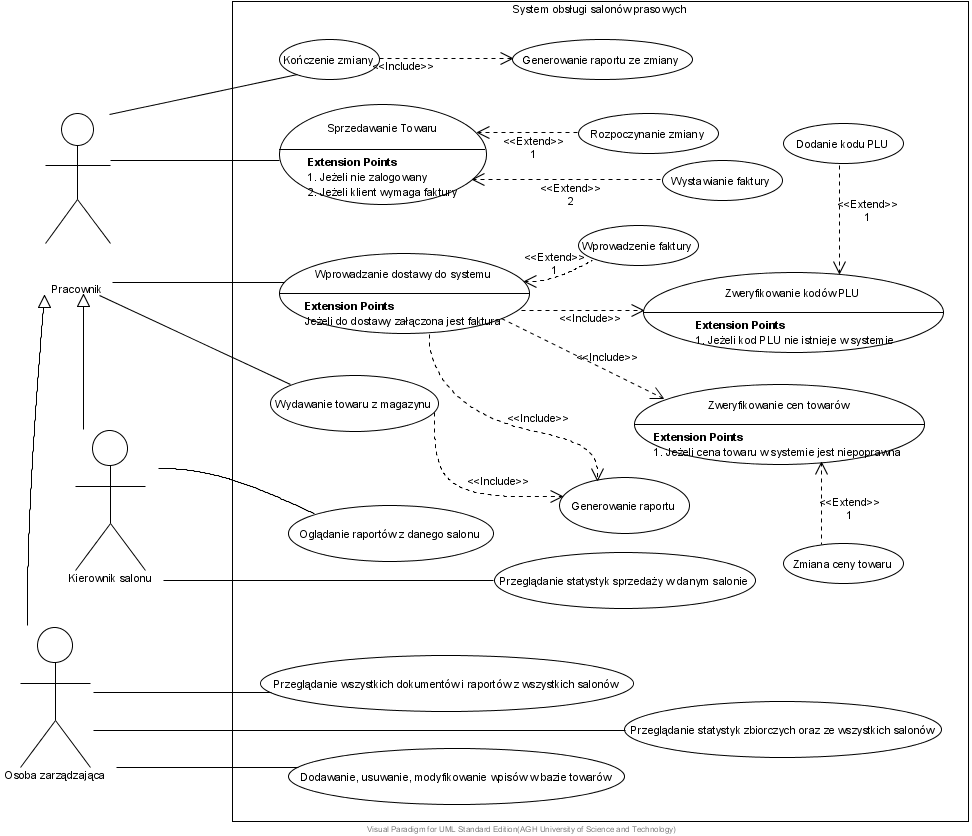
\includegraphics[width=1\textwidth]{gfx/usecase.png}
\caption{Diagram przypadków użycia systemu}
\end{figure}
\clearpage
\subsection{Diagram kontekstowy (przepływu danych - poziom 0)}
\begin{figure}[h]
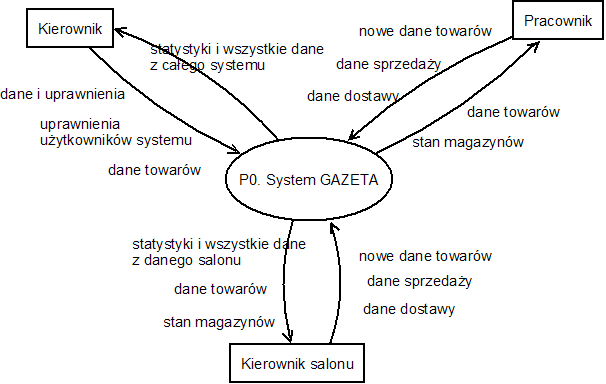
\includegraphics[width=1\textwidth]{gfx/dfd-0.png}
\caption{DFD - poziom 0 (diagram kontekstowy)}
\end{figure}
\clearpage
\subsection{Diagram przepływu danych - poziom 1}
\begin{figure}[h]
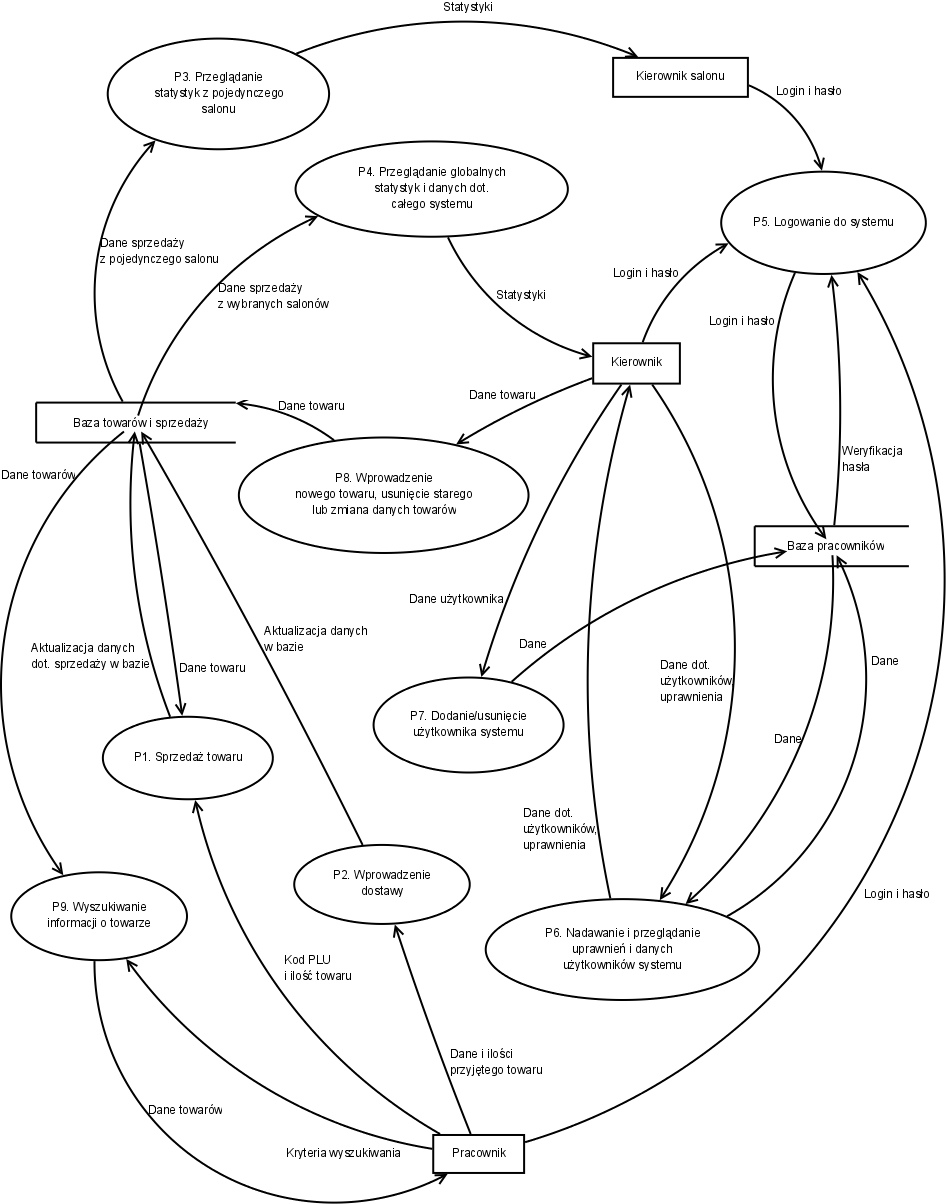
\includegraphics[width=1\textwidth]{gfx/dfd-1.png}
\caption{DFD - poziom 1}
\end{figure}
\clearpage
\subsection{Diagramy przepływu danych - poziom 2}
\subsubsection{Poziom 2.1 - Sprzedaż towaru}
\begin{figure}[h]
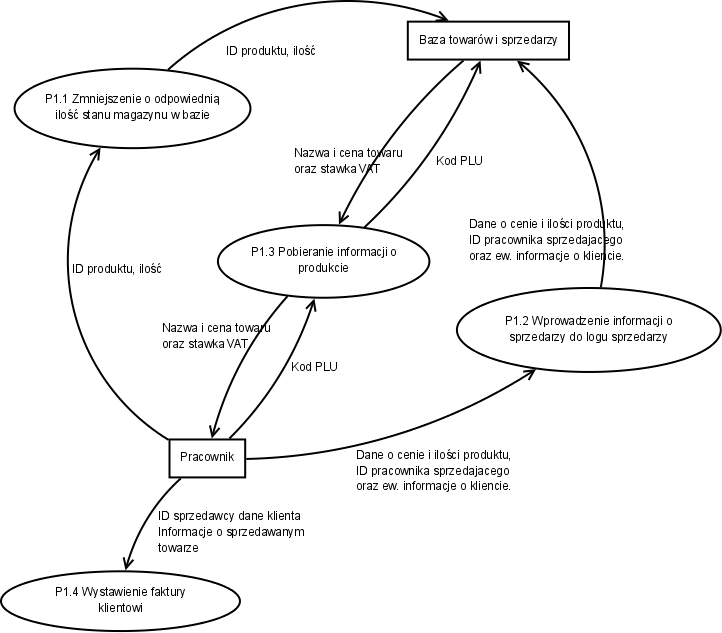
\includegraphics[width=1\textwidth]{gfx/dfd-2-1.png}
\caption{DFD - poziom 2.1 - Sprzedaż towaru}
\end{figure}
\clearpage
\subsubsection{Poziom 2.2 - Wprowadzenie dostawy}
\begin{figure}[h]
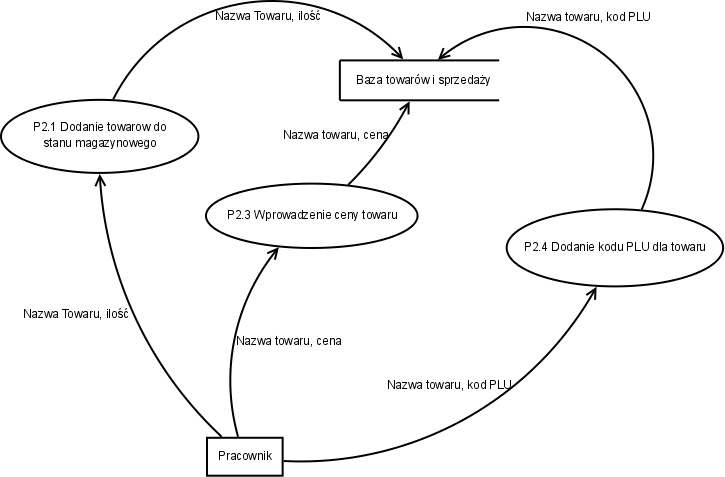
\includegraphics[width=1\textwidth]{gfx/dfd-2-2.png}
\caption{DFD - poziom 2.2 - Wprowadzenie dostawy}
\end{figure}
\clearpage
\subsubsection{Poziom 2.3 - Przeglądanie statystyk salonu}
\begin{figure}[h]
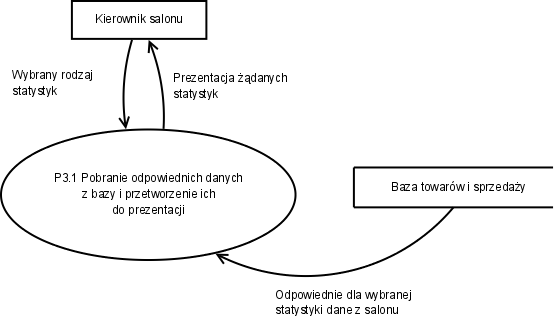
\includegraphics[width=1\textwidth]{gfx/dfd-2-3.png}
\caption{DFD - poziom 2.3 - Przeglądanie statystyk salonu}
\end{figure}
\clearpage
\subsubsection{Poziom 2.4 - Przeglądanie statystyk globalnych}
\begin{figure}[h]
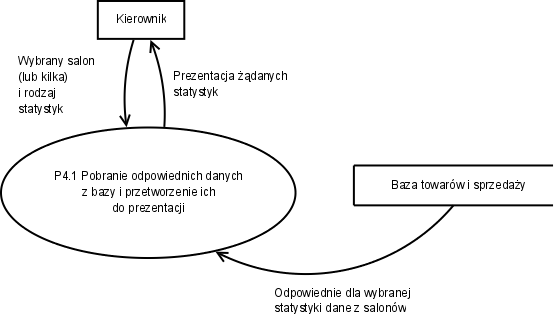
\includegraphics[width=1\textwidth]{gfx/dfd-2-4.png}
\caption{DFD - poziom 2.4 - Przeglądanie statystyk globalnych}
\end{figure}
\clearpage
\subsubsection{Poziom 2.5 - Logowanie do systemu}
\begin{figure}[h]
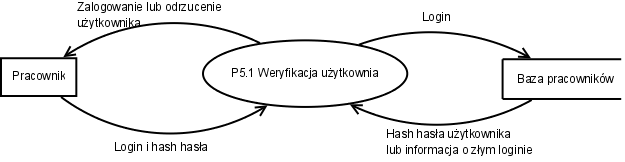
\includegraphics[width=1\textwidth]{gfx/dfd-2-5.png}
\caption{DFD - poziom 2.5 - Logowanie do systemu}
\end{figure}
\clearpage
\subsubsection{Poziom 2.6 - Nadawanie i przeglądanie uprawnień i danych użytkowników systemu}
\begin{figure}[h]
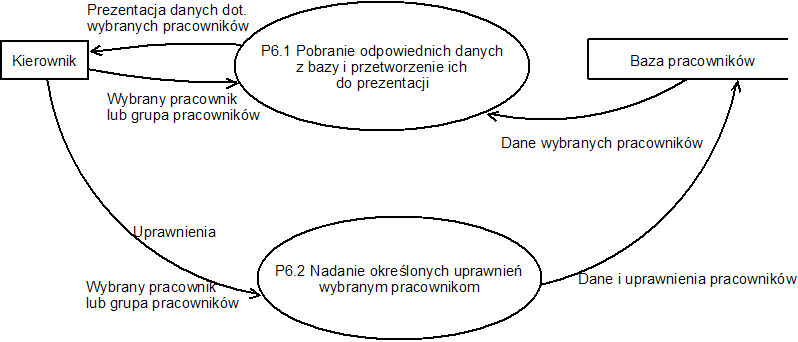
\includegraphics[width=1\textwidth]{gfx/dfd-2-6.png}
\caption{DFD - poziom 2.6 - Nadawanie i przeglądanie uprawnień i danych użytkowników systemu}
\end{figure}
\clearpage
\subsubsection{Poziom 2.7 - Dodanie/usunięcie użytkownika systemu}
\begin{figure}[h]
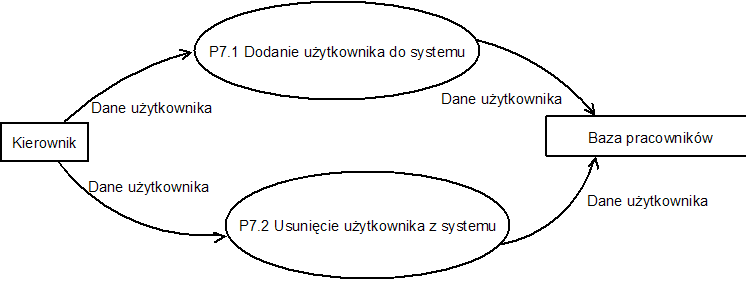
\includegraphics[width=1\textwidth]{gfx/dfd-2-7.png}
\caption{DFD - poziom 2.7 - Dodanie/usunięcie użytkownika systemu}
\end{figure}
\clearpage
\subsubsection{Poziom 2.8 - Wprowadzenie nowego towaru, usunięcie starego lub zmiana danych towarów}
\begin{figure}[h]
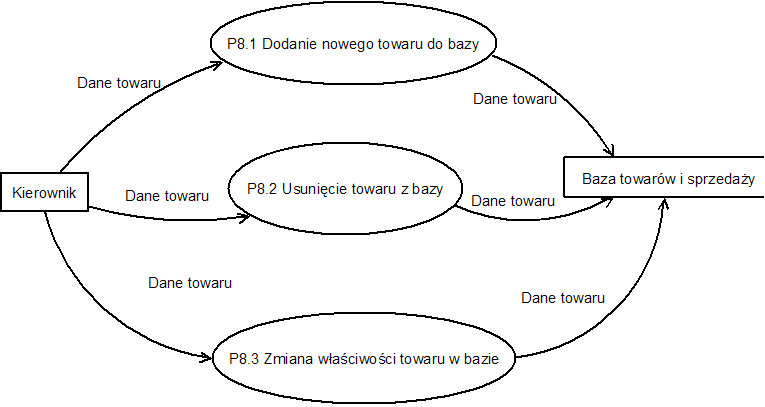
\includegraphics[width=1\textwidth]{gfx/dfd-2-8.png}
\caption{DFD - poziom 2.8 - Wprowadzenie nowego towaru, usunięcie starego lub zmiana danych towarów}
\end{figure}
\clearpage
\subsubsection{Poziom 2.9 - Wyszukiwanie informacji o towarze}
\begin{figure}[h]
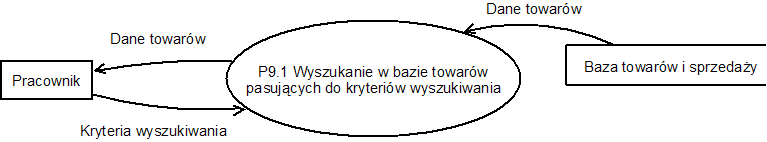
\includegraphics[width=1\textwidth]{gfx/dfd-2-9.png}
\caption{DFD - poziom 2.9 - Wyszukiwanie informacji o towarze}
\end{figure}
\clearpage
\subsection{Opisy procesów}
\subsubsection{Proces P1 - Sprzedaż towaru}
\begin{description}
\item[Proces P1.1 - Zmniejszenie o~odpowiednią ilość stanu magazynu] ~\\*
Sprzedanie towaru musi skutkować zmniejszeniem, o~ilość adekwatną do ilości sprzedanego towaru, ilości danego towaru w~bazie danych. Próba sprzedania większej ilości towaru niż znajduje się w~magazynie, a~co za tym idzie w~bazie, skutkuje wyświetleniem komunikatu z~informacją o~niemożności zrealizowania transakcji i~zatrzymanie sprzedaży.
\item[Proces P1.2 - Wprowadzenie informacji o~sprzedaży do logu sprzedaży] ~\\*
Po dokonaniu sprzedaży towaru, informacje o~tym zdarzeniu należy zapisać do tablicy logów. Wpis taki powinien zawierać:
\begin{itemize}
\item numer salonu
\item identyfikator sprzedającego pracownika
\item identyfikator klienta o~ile klientowi wystawiana jest faktura
\item identyfikator towaru
\item ilość towaru
\item cena jednostkowa
\item data i~czas sprzedaży.
\end{itemize}
\item[Proces P1.3 - Pobieranie informacji o~produkcie]  ~\\*
Informacje potrzebne do dokonania transakcji należy pobrać z~bazy danych na podstawie kodu PLU przekazanego do systemu przez czytnik kodów kreskowych. W~szczególności z~bazy należy pobrać
\begin{itemize}
\item nazwę towaru
\item cenę jednostkową
\item dostępną ilość towaru
\item stawkę VAT
\end{itemize}
odpowiadające towarowi o~danym PLU.
\item[Proces P1.4 - Wystawienie faktury klientowi]  ~\\*
Sprzedawca dysponując danymi klienta sprawdza, czy klient o~takich danych jest już wprowadzony do systemu. Jeżeli tak, to potwierdza poprawność danych, koryguje je w~razie potrzeby i~wystawia fakturę dla tego klienta na kwotę i~towar zgodny ze sprzedanym. Jeżeli dane klienta nie znajdują się w~systemie, sprzedawca wprowadza dane klienta do systemu i~drukuje fakturę dla nowo utworzonego klienta.
\end{description}
\subsubsection{Proces P2 - Wprowadzenie dostawy}
\begin{description}
\item[Proces P2.1 - Dodanie towarów do stanu magazynowego] ~\\*
Pracownik, odbierając dostawę towaru, zwiększa ilość danego towaru w~bazie danych. Towar rozpoznawany jest za pomocą jego kodu kreskowego, tak więc zadanie pracownika ogranicza się od sczytania kodu PLU towaru i~wprowadzenia liczby dostarczonych sztuk. Informacja o~dodaniu towaru powinna być odnotowana w~logu magazynowym i~powinna zawierać:
\begin{itemize}
\item identyfikator saloniku
\item identyfikator pracownika przyjmującego i~wprowadzającego dostawę
\item identyfikator produktu
\item wielkość dostawy (ilość sztuk)
\item czas wprowadzenia dostawy
\end{itemize}
\item[Proces P2.2 - Wprowadzenie ceny towaru] ~\\*
W~przypadku kiedy dostarczony towar należy sprzedawać w~innej cenie niż cena wprowadzona w~systemie (np. prasa przyszła z~nadrukowaną inną ceną niż dotychczas) pracownik zmienia cenę danego towaru dla swojego salonu w~systemie. Informacja o~zmianie ceny jest odnotowywana w~bazie wraz z~informacją o~czasie zmiany oraz o~osobie dokonującej tej zmiany.
\item[Proces P2.3 - Dodanie kodu PLU do towaru] ~\\*
W~przypadku kiedy dostarczony towar ma kod PLU, nierozpoznawany przez system (czasami towar przychodzi z~nowym kodem PLU), pracownik wyszukuje towar w~bazie danych po jego nazwie, a~następnie dodaje nowy PLU dla tego towaru. PLU nowego towaru rozpoznawany jest za pomocą czytnika kodów kreskowych.
\end{description}
\subsubsection{Proces P3 - Przeglądanie statystyk salonu}
\begin{description}
\item[Proces P3.1 - Pobranie odpowiednich danych z bazy i~przetworzenie ich do prezentacji] ~\\*
Kierownik salonu oraz osoba zarządzająca siecią saloników mają możliwość przeglądania wybranego przez siebie rodzaju statystyk dotyczących funkcjonowania danego saloniku. Statystyki powinny być prezentowane w postaci wykresów słupkowych. Dostępne są następujące rodzaje statystyk:
\begin{description}
\item[Statystyki sprzedaży towaru] opisujące ilość sprzedanego wybranego towaru w ujęciu dziennym, miesięcznym lub rocznym, wraz z ilością sprzedanego towaru podana jest też wartość sprzedaży. Dodatkowo dostępna jest statystyka przedstawiająca rozkład ilości sprzedanego towaru w ujęciu miesięcznym, tygodniowym i dziennym w ustalonym okresie czasu (np. procentowy rozkład sprzedaży danego towaru w ciągu dnia z podziałem na godziny, biorąc pod uwagę ostatni miesiąc, albo procentowy rozkład sprzedaży w ciągu tygodnia z podziałem na dni tygodnia biorąc pod uwagę dane ze sprzedaży z ostatnich 25 dni.
\item[Statystyki sprzedaży] opisujące całkowitą ilość sprzedanego towaru w wyznaczonym okresie czasu, wartość tej sprzedaży, a także rankingi towarów wg. ilości sprzedanych sztuk oraz wartości tej sprzedaży.
\item[Statystyki zmian] opisujące sprzedaż (ilość, wartość) pogrupowane wg. godzin zmiany (poranna, popołudniowa, wieczorna) lub wg. pracowników z wybranego okresu czasu
\end{description}
Ponadto, możliwe jest przeglądanie raportów z pracy saloniku, w tym:
\begin{description}
\item[Raporty ze zmian] zawierające podsumowania kolejnych zmian pracowników
\item[Raporty dzienne] zawierające podsumowanie całodziennej działalności saloniku
\item[Raporty o zmianach cen] zawierające informacje o zmianach cen wprowadzonych przez pracownika przy odbieraniu dostawy
\end{description}
\end{description}
\subsubsection{Proces P4 - Przeglądanie statystyk globalnych}
\begin{description}
\item[Proces P4.1 - Pobranie odpowienich danych z bazy i~przetworzenie ich do prezentacji] ~\\*
Osoba zarządzająca siecią ma możliwość przeglądania statystyk wygenerowanych nie dla jednego salonu, lecz zagregowanych dla kilku saloników lub dla całej sieci. Format takich statystyk identyczny jest do formatu statystyk dla pojedynczego salonu. Ponadto dostępne są też statystyki porównawcze salonów, w tym:
\begin{description}
\item[Statystyki sprzedaży] opisujące wielkość i wartość sprzedaży saloniku w porównaniu z innymi oraz ranking najlepszych saloników
\item[Statystyki sprzedaży towarów] opisujące wielkość i wartość sprzedaży danego towaru w porównaniu z innymi salonikami w podanym okresie czasu
\end{description}
Ponadto, osoba zarządzająca ma wgląd do raportów wygenerowanych przez wszystkie saloniki, w szczególności do raportów informujących o zmianach cen wprowadzonych przez pracowników w czasie dostawy towaru.
\end{description}
\subsubsection{Proces P5 - Logowanie do systemu}
\begin{description}
\item[Proces P5.1 - Weryfikacja użytkownika] ~\\*
\end{description}
Każdy z pracowników (wyróżniamy 3 poziomy uprawnień: pracownik, kierownik saloniku oraz kierownik całej sieci saloników.k) przed rozpoczęciem pracy z systemem musi się do niego zalogować. Procedura ta przebiega standardowo, użytkownik wpisuje login oraz hasło. Z bazy danych zostaje pobrana suma kontrolna hasła, przy pomocy której system weryfikuje poprawność logowania użytkownika. W zależności od wyniku weryfikacji, użytkownik zostaje zalogowany do systemu, bądź pojawia się komunikat o niepoprawnym logowaniu. Każde logowanie zostaje zapisane w bazie danych, i rozpoczyna zmianę pracownika. Pracownik, który obsługuje kasę, odpowiada za jej stan przez czas, przez który jest na niej zalogowany.
\subsubsection{Proces P6 - Nadawanie i przeglądanie uprawnień i danych użytkowników systemu}
\begin{description}
\item[Proces P6.1 - Pobieranie odpowiednich danych z bazy i przetworzenie ich do prezentacji] ~\\*
Kierownik saloniku oraz osoba zarządzająca siecią ma możliwość przeglądania danych wszystkich pracowników, jacy jemu podlegają. W szczególności osoba zarządzająca może przeglądać dane wszystkich pracowników jak również pracowników z jednego bądź kilku wybranych saloników.
\item[Proces P6.2 - Nadanie określonych uprawnień wybranym pracownikom] ~\\*
Osoba zarządzająca siecią powinna nadać każdemu z pracowników uprawnienia oraz ma możliwość ich zmiany. Każdy z pracowników musi mieć przypisany salonik w którym pracuje oraz funkcję jaką pełni. Dane te muszą zostać uzupełnione przed pierwszym zalogowaniem, mogą być także zmieniane (pracownik może awansować na kierownika salonu). Wyróżniamy 3 poziomy uprawnień: pracownik, kierownik saloniku oraz kierownik całej sieci saloników.
\end{description}
\subsubsection{Proces P7 - Dodanie/usunięcie użytkownika systemu}
\begin{description}
\item[Proces P7.1 - Dodanie użytkownika do systemu] ~\\*
Osoba zarządzająca siecią ma możliwość dodawania nowych użytkowników do systemu, zarówno pracowników, jak i kierowników salonów. W przypadku, kiedy zatrudniono nowego pracownika, należy wprowadzić jego dane oraz salonik w którym pracuje. Wprowadzone dane są następnie zapisywane w bazie danych.
\item[Proces P7.2 - Usunięcie użytkownika z systemu] ~\\*
Osoba zarządzająca siecią ma możliwość usuwania użytkowników z systemu, zarówno pracowników, jak i kierowników salonów. W przypadku, kiedy pracownik został zwolniony, należy wyszukać jego dane w systemie a następnie je usunąć. W następstwie tej akcji baza danych zostanie odpowiednio zaktualizowana.
\end{description}
\subsubsection{Proces P8 - Wprowadzenie nowego towaru, usunięcie starego lub zmiana danych towarów}
\begin{description}
\item[Proces P8.1 - Dodanie nowego towaru do bazy] ~\\*
Osoba zarządzająca siecią ma możliwość dodania nowego towaru do systemu. W przypadku, gdy w jednym z saloników (lub paru jest wprowadzony do sprzedaży nowy towar, należy wprowadzić jego dane, takie jak nazwa, cena, kod PLU, wartość podatku VAT oraz typ. Wprowadzone dane są następnie zapisywane w bazie danych.
\item[Proces P8.2 - Usunięcie towaru z bazy bazy] ~\\*
Osoba zarządzająca siecią ma możliwość usuwania istniejących towarów z systemu. W przypadku, kiedy dany towar nie będzie już więcej sprzedawany w żadnym z saloników, należy wyszukać dane tego towaru, a następnie wysłać do systemu żądanie usunięcia go. W następstwie tej akcji baza danych zostanie odpowiednio zaktualizowana.
\item[Proces P8.3 - Zmiana właściwości towaru w bazie] ~\\*
Osoba zarządzająca siecią ma możliwość zmiany danych istniejących towarów w systemie. W przypadku, kiedy na stałe zmienią się jakieś dane towaru, w szczególności towar nie będzie już identyfikowany pewnym kodem PLU, lub zostanie zmieniona jego cena, należy wyszukać dany towar w systemie, zmienić odpowiednio jego dane, oraz wysłać do systemu żądanie zmiany. Zmiany takie mogą wynikać z lokalnych zmian wprowadzonych w poszczególnych salonikach. W następstwie tej akcji baza danych zostanie odpowiednio zaktualizowana.
\end{description}
\subsubsection{Proces P8 - Wprowadzenie nowego towaru, usunięcie starego lub zmiana danych towarów}
\begin{description}
\item[Proces P9.1 - Wyszukiwanie informacji o towarze] ~\\*
Pracownik ma możliwość wyszukiwania danego towaru w bazie danych. Wyszukiwanie może odbywać się na podstawie fragmentu nazwy towaru, bądź też na podstawie kodu PLU (wprowadzonego np. z czytnika kodów kreskowych). Pracownik może też zdecydować czy chce w wyszukiwaniu uwzględnić tylko swój salonik czy poszukać towaru również w innych salonikach. Funkcja ta wykorzystywana może być do sprawdzenia ilości towaru na składzie saloniku, bądź też do sprawdzenia dostępności danego towaru w innych salonikach, jeżeli klientowi bardzo zależy na nabyciu towaru, który w danym saloniku jest niedostępny.
\end{description}
\section{Baza danych}
\begin{figure}
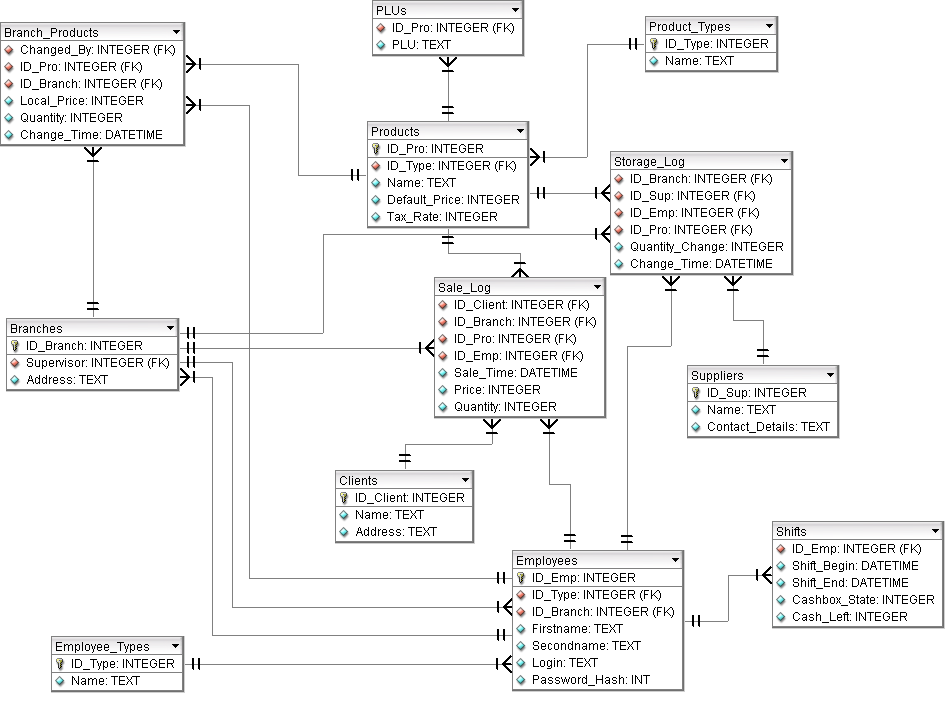
\includegraphics[width=1\textwidth]{gfx/baza.png}
\caption{Schemat bazy danych}
\end{figure}
Opis tabel:
\begin{description}
\item[Branches] każdy rekord tabeli odpowiada jednemu salonowi
    \begin{description}
    \item[ID\_Branch] - identyfikator salonu (klucz główny)
    \item[Supervisor] - identyfikator kierownika salonu (klucz obcy do tabeli Employees)
    \item[Address] - adres salonu
    \end{description}
\item[Employees] dane pracowników
    \begin{description}
    \item[ID\_Emp] - identyfikator pracownika (klucz główny)
    \item[ID\_Branch] - identyfikator salonu, w którym pracuje dany pracownik (klucz obcy do tabeli Branches)
    \item[Firstname] - imię pracownika
    \item[Secondname] - nazwisko pracownika
    \item[Login] - nazwa pracownika w systemie
    \item[Password\_Hash] - skrót kryptograficzny hasła pracownika
    \end{description}
\item[Shifts] zmiany pracowników
    \begin{description}
    \item[ID\_Emp] - pracownik, którego dotyczy dana informacja o zmianie (klucz obcy do tabeli Employees)
    \item[Shift\_Begin] - czas rozpoczęcia zmiany
    \item[Shift\_End] - czas zakończenia zmiany
    \item[Cashbox\_State] - stan kasy na zakończenie zmiany
    \item[Cash\_Left] - wartość zasiłku pozostawionego kolejnej zmianie
    \end{description}
\item[Products] dane dotyczące produktów
    \begin{description}
    \item[ID\_Pro] - identyfikator produktu (klucz główny)
    \item[ID\_Type] - typ produktu (klucz obcy do tabeli Product\_Types)
    \item[Name] - nazwa produktu
    \item[Default\_Price] - domyślna cena produktu
    \item[Tax\_Rate] - wartość podatku, jakim objęty jest produkt
    \end{description}
\item[Branch\_Products] dane dotyczące produktów, w konkretnych salonach
    \begin{description}
    \item[Changed\_By] - pracownik, wprowadzający zmianę (klucz obcy do tabeli Employees)
    \item[ID\_Pro] - identyfikator produktu (klucz obcy do tabeli Products)
    \item[ID\_Branch] - identyfikator salonu (klucz obcy do tabeli Branches)
    \item[Local\_Price] - cena produktu w salonie
    \item[Quantity] - ilość produktu dostępnego w salonie
    \end{description}
\item[Sale\_Log] dziennik sprzedaży
    \begin{description}
    \item[ID\_Client] - identyfikator klienta otrzymującego fakturę lub NULL, jeżeli faktura nie została wydana (klucz obcy do tabeli Clients)
    \item[ID\_Branch] - salon, w którym nastąpiła sprzedaż (klucz obcy do tabeli Branches)
    \item[ID\_Pro] - sprzedawany produkt (klucz obcy do tabeli Products)
    \item[ID\_Emp] - pracownik odpowiedzialny za sprzedaż (klucz obcy do tabeli Employees)
    \item[Sale\_Time] - czas sprzedaży
    \item[Price] - cena
    \item[Quantity] - ilość
    \end{description}
\item[Storage\_Log] dziennik operacji na magazynie
    \begin{description}
    \item[ID\_Branch] - salon, którego dotyczy operacja (klucz obcy do tabeli Branches)
    \item[ID\_Sup] - identyfikator dostawcy (klucz obcy do tabeli Suppliers)
    \item[ID\_Emp] - pracownik odpowiedzialny za operację (klucz obcy do tabeli Employees)
    \item[ID\_Pro] - produkt, którego dotyczy operacja (klucz obcy do tabeli Products)
    \item[Quantity\_Change] - zmiana ilości stanu magazynu, wartość dodatnia oznacza przyjęcie towaru, ujemna --- wydanie
    \item[Change\_Time] - czas wykonania operacji
    \end{description}
\item[Product\_Types] typy produktów
    \begin{description}
    \item[ID\_Type] - identyfikator typu (klucz główny)
    \item[Name] - nazwa typu
    \end{description}
\item[Suppliers] dane dostawców
    \begin{description}
    \item[ID\_Sup] - identyfikator dostawcy (klucz główny)
    \item[Name] - nazwa dostawcy
    \item[Contact\_Details] - szczegóły dotyczące kontaktu z dostawcą
    \end{description}
\item[Clients] dane klientów (do faktur)
    \begin{description}
    \item[ID\_Client] - identyfikator klienta (klucz główny)
    \item[Name] - nazwa klienta
    \item[Address] - adres klienta
    \end{description}
\item[PLUs] kody PLU produktów
    \begin{description}
    \item[ID\_Pro] - identyfikator produktu (klucz obcy do tabeli Products)
    \item[PLU] - kod PLU
    \end{description}
\end{description}


\section{Architektura systemu}
\subsection{Ogólny zarys architektury}
System wykonany będzie w~oparciu o~architekturę klient -- serwer. Rolę klientów pełnić będą komputery znajdujące się z~salonikach, bądź też komputer używany przez osobę zarządzającą siecią salonów. Rolę serwera pełnić będzie serwer aplikacji, oraz komunikujący się z~nim serwer bazy danych. W~każdym z~saloników, do komputera podłączona będzie kasa fiskalna, przeznaczona do prowadzenia sprzedaży oraz drukarka wykorzystywana do drukowania faktur dla klientów oraz raportów dla kierownika salonu.
\begin{figure}
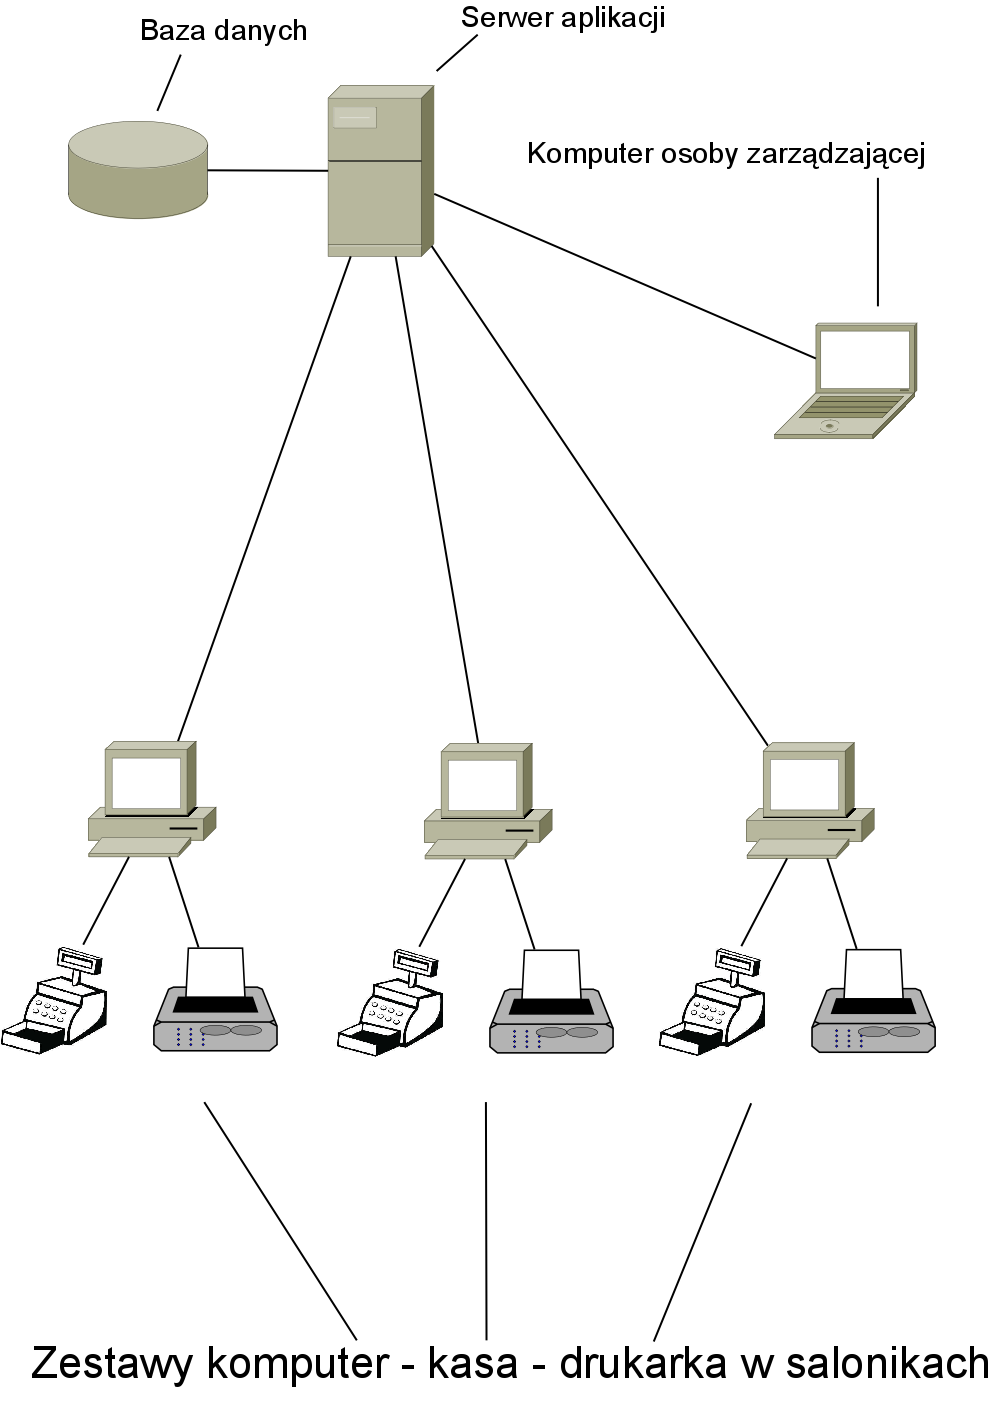
\includegraphics[width=1\textwidth]{gfx/architektura.png}
\caption{Ogólny zarys architektury systemu}
\end{figure}
\subsection{Platforma systemowa}
Zarówno serwer jak i~klient systemu napisane zostaną z~wykorzystaniem technologii Java 1.6. Komputery--klienty pracować będą pod kontrolą systemu operacyjnego Windows XP\texttrademark ,~natomiast serwer aplikacji uruchomiony będzie pod kontrolą systemu Linux. Baza danych wykorzystywana przez system działać będzie w~systemie PostreSQL, a~połączenie z~bazą będzie możliwe tylko z~serwera aplikacji.
\subsection{Komunikacja}
\subsubsection{Połączenie}
Każdy klient podłączać się będzie do serwera poprzez łącze internetowe dostępne w~saloniku (ADSL lub GPRS). Klient będzie podłączony do serwera co najmniej tak długo, jak długo trwać będzie praca salonu. Podłączenie do serwera możliwe będzie jedynie, gdy klient posiadać będzie odpowiedni identyfikator, zależny od salonika skojarzonego z~tym klientem oraz klucz, który będzie regularnie zmieniany bez ingerencji użytkownika podczas pracy systemu. Wszystkie próby (zarówno udane jak i~nie udane) serwer powinien odnotować w~swoich logach.
\subsubsection{Bezpieczeństwo}
Wszelka komunikacja pomiędzy serwerem, a~klientem odbywać się będzie za pośrednictwem szyfrowanego połączenia. Połączenie zestawiane będzie przy wykorzystaniu szyfru asymetrycznego, a~następnie wymieniony zostanie losowo wygenerowany klucz symetryczny, przy pomocy którego będzie się odbywało szyfrowanie i~deszyfrowanie przesyłanych danych.
\subsection{Kasa fiskalna}
%TODO: KUBO!!!! DO DZIEŁA!!!

\subsection{Przykładowy opis działania systemu}
\subsubsection{Zmiana ceny towaru przez kierownika sieci}
Kierownik sieci uruchamia na swoim komputerze klienta. Klient podłącza się do serwera aplikacji. Następnie kierownik, korzystając ze swojego loginu oraz hasła loguje się do systemu. Korzystając z~interfejsu udostępnionego przez klienta, zmienia cenę towaru X. Informacja o~żądaniu zmiany towaru jest przesyłana do serwera, a~ten wprowadza poprawkę do bazy danych. Serwer sprawdza też, w~ofercie których saloników znajduje się towar o~zmienionej właśnie cenie. Następnie, do klientów odpowiadających tym salonikom, w~którym towar się znajduje, wysyłana jest informacja o~zmianie tej ceny. Jeżeli dany klient jest w~tej chwili nie osiągalny (nie jest podłączony do systemu, np. z~powodu awarii łącza w~saloniku), wiadomość o~zmianie ceny zostaje dodana do kolejki wiadomości przeznaczonych dla tego klienta. Klient w~momencie odebrania takiej informacji, pobiera z~serwera aktualną bazę informacji o~cenach i~produktach znajdujących się w~ofercie danego saloniku, a~następnie aktualne dane automatycznie wprowadzane są do kasy.
\subsubsection{Sprzedaż towaru w~saloniku}
Pracownik saloniku, rozpoczynając swoją zmianę, loguje się do systemu wykorzystując swój login i~hasło. W~momencie zatwierdzenia sprzedaży na kasie, informacja o~sprzedanych towarach wysyłana jest z~kasy do klienta. Klient propaguje tą informację do serwera dołączając wzbogacając ją dodatkowo o~informacje na temat identyfikatora sprzedającego, czy czasu sprzedaży.

%spis ilustracji i~tabel
\clearpage
\listoffigures
%\listoftables
\end{document}

